\documentclass[a4paper]{scrartcl}
\usepackage[utf8]{inputenc}  
\usepackage[T1]{fontenc}
\usepackage{lmodern}           
\usepackage[ngerman]{babel}

% Was wir vielleicht brauchen koennten:
%\usepackage{amsmath} % More math.
%\usepackage[perpage,bottom]{footmisc} % Footnote configuration.

% Was wir ziemlich sicher brauchen:
\usepackage{fancyhdr} % For header and footer format
%\usepackage{fancyref} % For fancy references
\usepackage{listings} % For code listings
\usepackage{booktabs} % For tables
\usepackage[perpage,bottom]{footmisc} % Footnote configuration
\usepackage{graphicx} % For includegraphics
\usepackage[page,titletoc]{appendix} % For appendix in toc
\usepackage{color} % For colors, not sure if I truly need it anymore
\usepackage{caption} % For nicer listing captions
\usepackage{xspace} % For horizontal space.
\usepackage{pst-gantt} % For GANTT chart.

% Keine Ahnung warum, aber "`bla"' funktioniert bei mir nicht.
\newcommand{\enquote}[1]{\glqq{}#1\grqq{}}

% Big O
\newcommand{\bigO}{\ensuremath{\mathcal{O}}}

% Hyperref macht Links hinter die Sections und manipuliert PDF-Metadaten:
\usepackage[
colorlinks=false,
pdfborder={0 0 0},
pdftitle={Zufällige Polygone und kürzeste Wege},
pdfsubject={Abschlussbericht zum Softwareprojekt \enquote{Zufällige Polygone und kürzeste Wege}},
pdfauthor={Steve Dierker, Marcel Ehrhardt, Jannis Ihrig, Malte Rohde, Sebastian Thobe, Kadir Tugan}
%pdfkeywords={}
]{hyperref}

% Pimp my listings environment.
% Credits go to stackoverflow:
% http://stackoverflow.com/questions/741985/latex-source-code-listing-like-in-professional-books
\lstset{
         basicstyle=\footnotesize\ttfamily, % Standardschrift
         numberstyle=\tiny,          % Stil der Zeilennummern
         numbers=left,
         stepnumber=1,
         numbersep=7pt,              % Abstand der Nummern zum Text
         keywordstyle=\bfseries\ttfamily,
         tabsize=2,                  % Groesse von Tabs
         extendedchars=true,         %
         breaklines=true,            % Zeilen werden Umgebrochen       
         showspaces=false,           % Leerzeichen anzeigen ?
         showtabs=false,             % Tabs anzeigen ?
         %frame=b,                   % Linie unten
         breakatwhitespace=true,
         xleftmargin=17pt,
         framexleftmargin=17pt,
         framexrightmargin=5pt,
         framexbottommargin=4pt,
         showstringspaces=false      % Leerzeichen in Strings anzeigen ?      
 }

% Pimp my captions.
\DeclareCaptionFont{white}{\color{white}}
\DeclareCaptionFormat{listing}{\colorbox[cmyk]{0.43, 0.35, 0.35,0.01}{\parbox{\textwidth}{\hspace{15pt}#1#2#3}}}
\captionsetup[lstlisting]{format=listing,labelfont=white,textfont=white, singlelinecheck=false, margin=0pt, font={bf}}
%\DeclareCaptionFormat{figure}{\colorbox[cmyk]{0.43, 0.35, 0.35,0.01}{\parbox{\textwidth}{\hspace{15pt}#1#2#3}}}
%\captionsetup[figure]{format=listing,labelfont=white,textfont=white, singlelinecheck=false, margin=0pt, font={bf,footnotesize}}
%\DeclareCaptionFormat{table}{\colorbox[cmyk]{0.43, 0.35, 0.35,0.01}{\parbox{\textwidth}{\hspace{15pt}#1#2#3}}}
%\captionsetup[table]{format=listing,labelfont=white,textfont=white, singlelinecheck=false, margin=0pt, font={bf,footnotesize}}

% Listing environment for C
\lstnewenvironment{code}[1][]
  {\minipage{\linewidth} 
   \lstset{language=C,#1}}
  {\endminipage}

% Konfiguration der Titelseite:
\title{
{\normalsize Softwareprojekt über Anwendung effizienter Algorithmen\\ Wintersemester 2011/12}
\\[4ex] 
{\Large Abschlussbericht zum Softwareprojekt\\ \enquote{Zufällige Polygone und kürzeste Wege}}
\\[6ex]
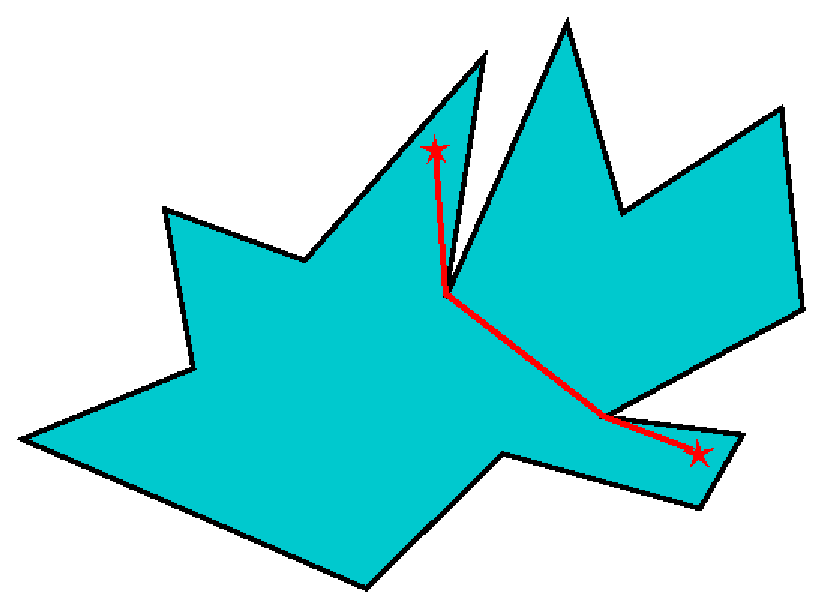
\includegraphics[width=0.4\textwidth]{img/polygons}
\\[3.5cm]}
\author{Steve Dierker \and Marcel Ehrhardt \and Jannis Ihrig \and Malte Rohde \and Sebastian Thobe \and Kadir Tugan}

\date{\vspace{2.5cm} \today{}}

\begin{document}

\begin{titlepage}
\pagenumbering{alph}
\maketitle
\thispagestyle{empty}
\vfill{}
\end{titlepage}

\pagestyle{empty}
\pagenumbering{roman}
%\include{parts/abstract}
\tableofcontents
\clearpage

\pagenumbering{arabic}
\pagestyle{fancy}
\setcounter{page}{1}

% Hier hin unsere Kapitel.
\section{Einleitung}

  Die algorithmische Geometrie als Teilgebiet der Informatik beschäftigt sich
  mit der algorithmischen Lösung geometrischer Probleme. Einfache Polygone
  (überschneidungsfreie, zusammenhängende, planare Vielecke) bilden die
  Grundlage vieler Aufgabengebiete der algorithmischen Geometrie. Als
  naheliegendes Beispiel bezeichnet die Triangulierung die Zerlegung eines
  Polygons in eine Menge von Dreiecken, die die Fläche des Polygons
  überdecken. Diese Dreieckszerlegung ermöglicht die Lösung einer ganzen Reihe
  weiterer geometrische Probleme.

  Zum Testen und zur Evaluation polygon-basierter geometrischer
  Algorithmen ist es oft von Vorteil, über eine beliebige Menge einfacher
  Polygone zu verfügen, wobei diese, um eine gewisse Aussagekraft der
  Experimente zu gewährleisten, möglichst alle (in einem
  definierten planaren Raum) vorstellbaren Polygone erzeugen können sollten. Die
  massenweise Erzeugung solcher \emph{zufälliger Polygone} ist ein
  Forschungsgebiet, dem in den vergangenen Jahrzehnten daher vermehrt
  wissenschaftliche Aufmerksamkeit zugekommen ist. Die entstandenen
  Lösungswege und Algorithmen unterscheiden sich unter anderem in ihrer
  Komplexität, im Speicherverbrauch sowie in der Art und
  \enquote{Zufälligkeit} der erzeugten Polygone.

  Der vorliegende Text ist der Abschlussbericht des Softwareprojekts
  \emph{Zufällige Polygone und kürzeste Wege}, welches im Rahmen des Moduls
  \enquote{Softwareprojekt: Anwendung von Algorithmen} unter Leitung von Prof.
  Dr. Günter Rote durchgeführt wurde. Das Ziel des Projekts war die
  Entwicklung einer Softwarebibliothek, welche über verschiedenene Algorithmen
  zur Erzeugung zufälliger Polygone verfügen und diese unter anderem
  über eine grafische Schnittstelle dem Benutzer zur Verfügung stellen sollte.
  Das Projekt wurde mit Ende des Wintersemesters 2011/2012 abgeschlossen.

  Im Folgenden werden wir zunächst die Zielsetzung des Projekts, funktionale
  und nicht-funktionale Anforderungen an die zu implementierende Software,
  sowie Einschränkungen der Zielsetzung darstellen. Anschließend erfolgt eine
  kurze Erläuterung des von uns gewählten Entwicklungsprozesses und dessen
  Umsetzung. Im Hauptteil des Berichts gehen wir detailliert auf die
  Eigenschaften der einzelnen Algorithmen sowie auf die während der
  Entwicklung aufgetretenden Probleme und deren Lösungen ein. In
  Kapitel~\ref{sec:manual} findet der Leser einen umfassenden
  \emph{Benutzerleitfaden} für die entstandene Softwarelösung. Im letzten
  Kapitel schließen wir den Bericht mit einem kurzen Fazit zum Projektablauf
  sowie zu unserer Einschätzung der Brauchbarkeit der Software.

\section{Projektstruktur}

  Das Projekt \emph{Zufällige Polygone} wurde im Wintersemester 2011/2012 in
  einem Zeitraum von rund 4 Monaten durchgeführt. Im Folgenden werden wir
  zunächst die Ziele des Projekts darstellen, den zeitlichen Ablauf darlegen
  und abschließend den gewählten Entwicklungsprozess beschreiben.

  \subsection{Zielsetzung \& Einschränkungen}

    Das Hauptziel des Projekts war die Implementierung einer Reihe von
    Algorithmen, die der Erzeugung zufälliger einfacher Polygone dienen. Vom
    verantwortlichen Dozenten wurden dabei vier wissenschaftliche Artikel zur
    Verfügung gestellt, in denen insgesamt 7 derartige Algorithmen beschrieben
    werden. Darüberhinaus sollte ein vom Dozenten mitentwickelter \emph
    {Shortest-Path}-Algorithmus~\cite{asano11shortestpath} implementiert werden,
    welcher in einem gegebenen Polygon die kürzeste Verbindung zwischen zwei
    gewählten Punkten errechnet. Folgende weitergehenden Anforderungen an die zu
    entwickelnde Software waren gegeben:

    \begin{itemize}
      \item Massenweise (\emph{batch}) Erzeugung von zufälligen Polygonen 
            per Kommandozeile
      \item Export eines oder vieler Polygone als CSV-Datei 
            (\emph{comma-separated value})
      \item Grafische Oberfläche
      \begin{itemize}
        \item Auswahl und Konfiguration des Algorithmus
        \item Visualisierung der Funktionsweise des Algorithmus
        \item Auswahl der Punkte für den Shortest-Path-Algorithmus
        \item Visualisierung der Funktionsweise des Shortest-Path-Algorithmus
      \end{itemize}
      \item Statistische Analyse der Algorithmen hinsichtlich ihrer Laufzeit 
            und den Eigenschaften der erzeugten Polygone
    \end{itemize}

    Als Programmiersprache wählten wir \emph{Java}, da alle Projektmitglieder
    über Erfahrung in der Java-Programmierung verfügten und die Sprache sowohl
    die gewünschte Performanz als auch eine ausreichend umfangreiche
    Standardbibliothek bot. Aufgrund des begrenzten zeitlichen Rahmens des
    Projekts mussten jedoch einige Einschränkungen in Bezug auf die
    mathematische Korrektheit der entwickelten Software getroffen werden.
    Zunächst ist hier die Entscheidung für die Verwendung von Gleitkomma- und
    gegen die (ausschließliche) Verwendung von Ganzzahlen zu nennen. Zwar
    ermöglichen Gleitkommazahlen die einfache und CPU-gestützte
    Divisionsoperation, jedoch kann es durch die begrenzte Auflösung der
    Gleitkommazahlen (bspw. 64 Bit bei Variablen des Typs \emph{double}) zu
    Rundungsungenauigkeiten kommen.

    Eine weitere, mithin gravierendere Einschränkung ist der Verzicht auf einen
    \emph{General Position}-Test (im Deutschen manchmal \enquote{allgemeine
    Lage}) vor Ausführung der Algorithmen. Eine Menge von Punkten in der Ebene
    befindet sich in \emph{general position}, wenn

    \begin{enumerate}
      \item keine zwei Punkte identisch sind,
      \item keine drei Punkte auf einer Geraden liegen und
      \item keine 4 Punkte auf einem Kreis liegen.
    \end{enumerate}

    Manche Polygon-Algorithmen versagen, wenn eine dieser Eigenschaften,
    insbesondere 2., für die gegebene Punktmenge nicht erfüllt ist. Zwar lässt
    sich eine Punktmenge leicht auf GP überprüfen, jedoch ist dieser Test vor
    allem für große Punktmengen sehr rechenintensiv. Der von uns vorübergehend
    verwendete naive Algorithmus zum GP-Test wies ein asymptotisches Wachstum
    von $\bigO\left(n^3\right)$ auf, sodass die Laufzeit des GP-Tests bisweilen
    die Laufzeit des Algorithmus weit übertraf. Als Konsequenz hieraus
    verzichteten wir auf einen GP-Test, sodass eine nicht in GP befindlichen
    Punktmenge zu undefinierte Ergebnissen des Programms führen kann. Mit der
    Verwendung von 64-bit \emph{double}-Variablen zur Darstellung der $x$- und
    $y$-Koordinaten ist eine solche Situation jedoch äußerst unwahrscheinlich.

  \subsection{Zeitplan}

    Wir präsentieren hier den Zeitplan des Projekts in Form eines GANTT-
    Diagramms, welches auch während der Projektarbeit Verwendung fand. Da das
    Diagramm laufend an den aktuellen Entwicklungsstand angepasst wurde,
    entspricht es nun nahezu exakt dem tatsächlichen zeitlichen Ablauf der
    Entwicklung.

    \begin{figure}[h]
    \begin{center}
    \bfseries\fontsize{5}{5}\selectfont
    \newpsstyle{TaskStyleA}{fillstyle=solid,fillcolor=red}
    \begin{PstGanttChart}[% 
        yunit=1.0,
        xunit=0.68,
        ChartUnitIntervalName=KW,
        ChartUnitBasicIntervalName=KW,
    %    ChartModulo,
        ChartModuloValue=52,
        TaskUnitIntervalValue=14,
        TaskUnitType=KW,
        ChartStartInterval=43,
        ChartShowIntervals]{15}{15}
    \psset{TaskStyle=TaskStyleA}
    \PstGanttTask[TaskInsideLabel={PolygonGenerator interface}]{0}{4}
    \PstGanttTask[TaskInsideLabel={Data structures scratch}]{0}{4}
    \PstGanttTask[TaskInsideLabel={GUI scratch}]{0}{4}
    \PstGanttTask[TaskInsideLabel={Data structures done}]{1}{3}
    \PstGanttTask[TaskInsideLabel={First polygon algorithms}]{1}{4}
    \PstGanttTask[TaskInsideLabel={ShortestPathGenerator interface}]{1}{4}
    \PstGanttTask[TaskInsideLabel={All polygon algorithms}]{3}{4}
    \PstGanttTask[TaskInsideLabel={Shortest path algorithm}]{3}{4}
    \PstGanttTask[TaskInsideLabel={GUI}]{3}{4}
    \PstGanttTask[TaskInsideLabel={History data structure}]{6}{4}
    \PstGanttTask[TaskInsideLabel={Step-by-step visualisation}]{6}{4}
    \PstGanttTask[TaskInsideLabel={Statistics backend}]{6}{4}
    \PstGanttTask[TaskInsideLabel={Improved GUI}]{10}{3}
    \PstGanttTask[TaskInsideLabel={Statistics visualisation}]{10}{3}
    \PstGanttTask[TaskInsideLabel={Cleanup for release}]{12}{3}
    \end{PstGanttChart}
    \end{center}
    \label{fig:gantt}
    \end{figure}

  \subsection{Entwicklungsprozess}

    Der von uns gewählte Entwicklungsprozess folgte keinem fest definierten
    Modell (bspw. SCRUM), beinhaltete jedoch einige prozessunterstützende
    Maßnahmen, die vor allem der kontinuierlichen Kommunikation innerhalb des
    Teams dienen sollten. Die folgenden Prozesselemente stellten sich als
    hilfreich heraus und wurden während der Projektarbeit konsequent
    beibehalten:

    \begin{itemize}
      \item Iterative Herangehensweise, stets lauffähige Version im Repository.
      \item Wöchentliche Team-Meetings zur Besprechung des aktuellen Stands, 
            der in der vergangenen Woche erledigten Arbeit sowie der für die 
            folgende Woche geplanten Arbeitspakete. Schriftliche Protokolle 
            dienten der Information abwesender Teammitglieder.
      \item Arbeitspakete werden stets in 2er-Teams bearbeitet, 
            unter anderem um den Busfaktor\footnote{\url{http://en.wikipedia.org/wiki/Bus_factor}} zu erhöhen.
      \item Unregelmäßig stattfindende \emph{coding sessions}.
    \end{itemize}

    Insbesondere der letztgenannte Punkt entwickelte sich im Laufe des Projekts
    zu einer wichtigen Maßnahme, um sowohl Verzögerungen im Zeitplan gering zu
    halten, als auch das Wissen über den geschriebenen Code möglichst
    gleichmäßig auf die Teammitglieder zu verteilen. Die \emph{coding sessions}
    wurden von allen Teammitgliedern als überaus produktiv empfunden, oftmals
    konnten an einem Tag eine ganze Reihe Arbeitspakete abgeschlossen werden.
    Zudem zeigten sich Fehler im Code oft erst, während mehrere, vorher
    unbeteiligte Teammitglieder den Code der anderen ausgiebig testeten.

    Entscheidungen im Team wurden weitestgehend per Konsens geschlossen. Für den
    seltenen Fall einer Unstimmigkeit wurde zuvor Jannis Ihrig zum Projektleiter
    bestimmt. Der Projektleiter vertrat das Projekt zudem als Ansprechpartner
    gegenüber dem Dozenten.

\section{Algorithmen zur Polygongenerierung}

  In Tabelle~\ref{algo_table} findet sich eine Auflistung der in der
  entstandenen Softwarelösung implementierten Algorithmen. Die meisten dieser
  Algorithmen bedürfen einer vorgegebenen Punktmenge, aus welcher ein simples
  Polygon konstruiert wird. Der \enquote{Random Polygon Algorithm} hingegen
  erhält als initialie Punktmenge lediglich die Eckpunkte eines Dreiecks und
  erzeugt im gegebenen begrenzten Raum eine konfigurierbare Anzahl weiterer
  Punkte. Der Algorithmus von Virmani verändert als einziger Algorithmus die
  Position der Punkte der vorgegebenen Punktmenge.

  Die in Tabelle~\ref{algo_table} angegebene \enquote{Laufzeit} bezeichnet die
  theoretisch kleinste obere Schranke für das asymptotische Wachstum der
  Laufzeitsfunktion der Algorithmen, in Abhängigkeit der Anzahl der Punkte $n$.
  In einigen Fällen lässt sich diese jedoch nicht bestimmen, bzw. beschreibt
  eine erwartete Laufzeit bei randomisierten Algorithmen (bspw. Permute \&
  Reject). Da die Laufzeit einiger Hilfsfunktionen (z.B. Polygon-Gerade-
  Schnittberechnung) in unserer Implementierung nicht ideal ist, weicht die
  Laufzeit der Algorithmen in der Implementierung zum Teil von der erwarteten
  Laufzeit ab.

  \begin{table}[ht]
    \begin{center}
    \caption{Polygon-Algorithmen}
    \begin{tabular}{lcc} 
      \toprule
      Algorithmus & erw. Laufzeit & Laufzeit (Impl.) \\
      \midrule
      Permute \& Reject & $\bigO(n!)$ & $\bigO(n!)$ \\
      Incremental Construction \& Backtracking & $\bigO(n!)$ & $\bigO(n!)$ \\
      Space Partitioning & $\bigO(n^2)$ & $\bigO(n^2)$\\
      Steady Growth & $\bigO(n^2)$ & ... \\
      2-Opt Moves & $\bigO(n^3)$ & $\bigO(n^4)$ \\
      Velocity Virmani & ... & ...\\
      Two Peasants & $\bigO(n \log n)$ & $\bigO(n \log n)$ \\
      Random Polygon Algorithm & $\bigO(n^2 \log n)$ & ... \\
      \bottomrule
    \end{tabular}
    \label{algo_table}
    \end{center}
  \end{table}

  Im Folgenden wird die Funktionsweise der einzelnen Algorithmen erläutert und
  auch besondere Eigenschaften der erzeugten Polygone dargestellt.

\subsection{Random Polygon Algorithm} % (fold)
\label{sub:random_polygon_algorithm}
	rpa

% subsection random_polygon_algorithm (end)

\subsection{Velocity Virmani}
Der Algorithmus \enquote{Velocity Virmani} wurde am 25. Juli 1991 in dem Paper \enquote{Generating Random Polygons} von Joseph O'Rourke und Mandira Virmani veröffentlicht \cite{virmani91polygons}.\smallskip \\ 
Er beschreibt einen Algorithmus zur Generierung zufälliger simpler Polygone mittels Verschiebungen von Punkten. In dem genannten Paper wurde dem Algorithmus kein Name gegeben, deshalb haben wir uns die Freiheit genommen und werden in unserer Ausarbeitung mit dem Namen \enquote{Velocity Virmani} oder \enquote{Virmani} darauf verweisen.

Der Algorithmus besteht aus 3 Kernkomponenten:
\begin{enumerate}
	\item Die Generierung von einem regulären Polygon with n Punkten
	\item Zufällige Verschiebungen der Eckpunkte
	\item Überprüfen ob das Polygon noch simpel ist
\end{enumerate}

\subsubsection{Generierung des regulären Polygons}
Eingabeparameter: 
\begin{itemize}
	\item Anzahl der Punkte(n)
	\item Radius(r)
\end{itemize}
Ausgabe:
\begin{itemize} 
	\item Reguläres Polygon mit n Punkten
\end{itemize}
Hier wird ein reguläres Polygon generiert indem ein Kreis genommen wird auf welchem n Punkte gleichmäßig verteilt werden und diese dann verbunden werden. Dazu wird der gesamte Kreisradius genommen(PI*2) und durch die Anzahl der Punkte geteilt(n): $winkel = (PI * 2) / n$.\\ 
Das Ergebnis ist der Abstand, als Winkel, zwischen jedem einzelnen Punkt.
Mit dem Radius zusammen kann man dann jeweiligen Koordinaten des regulären Polygons berechnen:\\
$x_i = r * cos(winkel * i)$\\
$y_i = r * sin(winkel * i)$

\subsubsection{Verschiebung}
Eingabeparameter: 
\begin{itemize}
	\item simples Polygon(polygon)
	\item Boundaries(boundary)
	\item maximale Geschwindigkeit(maxvelocity)
	\item Anzahl der Durchläufe (iterations)
\end{itemize}
Ausgabe:
\begin{itemize}
	\item Zufälliges Polygon
\end{itemize}
In diesem Teil wird jeder Punkt zufällig verschoben, die maximale Distanz pro Achse wird bestimmt durch den Eingabeparameter maxvelocity. Nach jeder Verschiebung von einem Punkt können folgende Zustände auftreten:
\begin{enumerate}
	\item Das Polygon ist simpel und in den Grenzen (Boundaries)
	\item Das Polygon ist simpel aber außerhalb der Grenzen
	\item Das Polygon ist nicht simpel aber innerhalb der Grenzen
	\item Das Polygon ist weder simpel noch in den Grenzen
\end{enumerate}
Sollte es vorkommen das der Zustand nicht Punkt 1 enspricht (simpel und in den Grenzen), so wird die Verschiebung rückgängig gemacht und für diesen Punkt im Polygon ändert sich nichts.
Dieser gesamte Prozess wird \enquote{iterations}-oft ausgeführt sodass es wirklich zufällig wird.

\paragraph{Pseudocode}

\begin{code}[mathescape=true]
for (int i=0; i < iterations; i++)
{
	foreach($p_i$ in polygon)
	{
		move_point_randomly($p_i$, maxvelocity);
		if(isSimple(polygon) && isInBound(polygon))
			continue;
		else
			revert_move_point_randomly($p_i$);
	}
}
\end{code}

\subsubsection{Überprüfen ob das Polygon simpel ist}
In dem Velocity Virmani wird nach jedem Punkt getestet ob das Polygon noch simpel ist. Dies kann bei einer trivialen Implementierung des Tests mit $n^3$ zu sehr hohen Laufzeiten führen.
Deshalb ist ein trivialer Test nach der Eigenschaft simpel nicht effizient.\smallskip \\ 
Die Lösung für dieses Problem besteht darin nur die angrenzenden Linien des verschobenen Punktes mit allen anderen Linien auf Überschneidungen zu überprüfen. Eine komplette Überprüfung auf Simplizität ist nicht nötig.
Der Algorithmus dafür wäre trivial sowie auch würde die Laufzeit für ein Test von $O(n^3)$ auf $O(n)$ sinken.

Vorraussetzung: Polygon muss vor der Verschiebung simpel sein
Eingabeparameter: Polygon, der verschobene Punkt(u)
Es werden die beiden zugehörigen Kanten von dem Punkt u genommen. Diese beiden Kanten werden mit den allen restlichen Kanten auf eine Schnittmenge überprüft. Sollte sich bei irgendeiner Kante eine Schnittmenge ergeben, so ist das Polygon nicht simpel und es muss nicht weiter getestet werden. Eine Ausnahme bilden jedoch die Endpunkte von den Kanten, jede Kante darf sich genau ein Endpunkt mit einer anderen Kante teilen.


\subsubsection{Eigenschaften}
\begin{itemize}
	\item Nichtdeterministisch\\
	Das Programm ist nichtdeterministisch da es ein Zufallsgenerator nutzt
	\item Komplexität: $O(iterations*n^2)$\\
	Die Komplexität setzt sich zusammen aus der Anzahl der Iterationen, aus der Anzahl der Punkte durch die Iteriert wird um die Verschiebungen durchzuführen sowie nochmal durch die Anzahl der Punkte für die Überprüfung ob es noch simpel ist. Somit ergibt sich eine Laufzeit von $O(iterations*n*n) = O(iterations*n^2)$
	\item Terminiert\\
	Der Algorithmus terminiert immer da die Anzahl der Schlaufendurchgänge begrenzt ist. Es gibt keinen Zustand im Algorithmus wo er verbleiben kann.
\end{itemize}

%TODO Überdenke diese Section und verkürze sie evtl.
%velocity <-> boundary box <-> radius <-> n
%velocity <-> radius
%space per point: boundary box <-> n
\subsection{Zufälligkeit der Polygone in Abhängigkeit von Parametern}
Der Algorithmus generiert zuverlässig zufällige Polygone bei der \enquote{richtigen} Eingabe von Parametern. Die Parameter haben diverse Abhängigkeiten untereinander in Bezug auf die Zufälligkeit des generierten Polygons:\\
\begin{itemize}
	\item maximale Geschwindigkeit <-> Boundary Box\\
	Die maximale Geschwindigkeit die ein Punkt pro Durchlauf annehmen kann ist abhängig von der Boundary Box. Es ist zum Beispiel nicht effektiv bei einer Boundary Box von 500x500 eine maximale Geschwindigkeit von 1000 festzulegen, da diese nicht erreicht werden kann. Der Effekt dabei ist das die Wahrscheinlichkeit das ein Punkt am Ende sich nicht bewegt weil es out of Bound ist, oder kollidiert, sehr hoch wird. Dadurch wird die Zufälligkeit des Polygons beeinflusst.\\
	Die maximale Geschwindigkeit zu klein zu setzen führt wiederrum dazu das man viele Iterationen braucht um mehr Weg bewältigen. Bei wenigen Iterationen würde somit das Polygon weniger zufällig sein.
	\item n <-> Boundary Box <-> maximale Geschwindigkeit\\
	Je größer die Anzahl der Punkte ist desto größer sollte die Boundary Box sein. Denn je mehr Punkte beisammen liegen, desto höher ist die Chance bei größeren Bewegungen das die Punkte \enquote{rejected} werden. Dies kann man Vorbeugen indem man die maximale Geschwindigkeit kleiner setzt. Jedoch sollte man auch hier Punkt 1 beachten.
	\item Radius <-> Boundary Box\\
	Das reguläre Polygon sollte so gesetzt werden das es mittig in der Boundary Box liegt. Idealerweise sollte die Entfernung von dem Polygon zur Boundary Box ungefähr dem Radius entsprechen.\\
	Der Grund dafür liegt darin das wenn die Boundary Box zu klein ist, das viele Bewegungen der Punkte welche nach außen gehen \enquote{rejected} werden.
	\item Radius <-> n\\
	Hier ist es wichtig das man nicht zuviele Punkte so dicht zusammenpackt. Das Problem ist wie bei den oben genannten Punkten das sonst sich die Punkte nicht frei bewegen können.
\end{itemize}
%TODO statt paragraph evtl. was anderes nutzen
\paragraph{Fazit}
Wie man sehen kann sind fast alle Parameter voneinander in gewisser Weise abhängig. Dies liegt daran das die folgenden Parameter jeweils den Raum der Punkte oder deren Bewegung bestimmen: n, boundary, maxvelocity, radius.\\
Der einzige Parameter der keine Abhängigkeit zu den Punkten oder zu dem Raum hat ist der Parameter \enquote{iterations}. Dieser Parameter kann bei genug hoher Festlegung dazu führen das selbst sehr ungünstig gesetzte Parameter zu einem guten, zufälligen Ergebnis führen.\\
Jedoch ist dies nicht empfehlenswert da Iterations einen starken Einfluss auf die Laufzeit hat und dies dazu führen kann das hohe Laufzeiten entstehen.
\subsection{Permute \& Reject}
\emph{Permute \& Reject} ist ein einfacher Algorithmus von Martin Held, zuerst beschrieben in~\cite{held98polygons}. Der Algorithmus basiert auf der zufälligen Erzeugung von $n$ Kanten zwischen $n$ gegebenen Punkten, sodass von jedem Punkt zwei Kanten ausgehen.
\subsubsection{Algorithmus}
\begin{code}[caption={Permute \& Reject},label=permutelisting,mathescape=true]
retry:
$P$ $\leftarrow$ given set of points
$p$ $\leftarrow$ remove random point from $P$
while ($P$ not empty)
  $q$ $\leftarrow$ remove random point from $P$
  draw edge from $p$ to $q$
  $p$ $\leftarrow$ $q$
if resulting polygon is NOT simple
  goto retry
\end{code}
\subsubsection{Eigenschaften}

\cleardoublepage
\phantomsection

% Bibliography
\addcontentsline{toc}{section}{Literatur}
\bibliographystyle{alpha}
\bibliography{report}

\end{document}
